% !TeX root = main.tex
%%%%%%%%%%%%%%%%%%%%%%%%% PREAMBLE %%%%%%%%%%%%%%%%%%%%%%%%%%%%%%%%
%%%%%%%%%%%%%%%%%%%%%%%% BASIC DOCUMENT SETUP %%%%%%%%%%%%%%%%%%%%%
\documentclass[a4paper]{report}
\usepackage[utf8]{inputenc}
\usepackage[english]{babel}

%%%%%%%%%%%%%%%%%%%%%%%%%% PACKAGES %%%%%%%%%%%%%%%%%%%%%%%%%%%%%%%
\usepackage{datetime}
\usepackage{datenumber}
\usepackage{parskip}
\usepackage{forest}
\usepackage{svg}        % makes it possible to use svg files
\usepackage{graphics}
\usepackage{multicol}
\usepackage{icomma}
\usepackage{microtype}  % microscopic typography refinement
\usepackage{lastpage}   % used to reference last page in footer
\usepackage{fancyhdr}   % Header
\usepackage{tcolorbox}
\usepackage{amssymb}
\usepackage[Bjornstrup]{fncychap}
\usepackage[titles]{tocloft}
\usepackage{amsmath}    % mathematics for matrices and more
\usepackage{amsfonts}
\usepackage{csquotes}
\usepackage{morewrites}

\usepackage{tikz}
\usetikzlibrary{calc}   % position og tikz labels
\usetikzlibrary{arrows.meta}
\usetikzlibrary{decorations.pathreplacing,calligraphy}

\usepackage{float}
\usepackage{pgfplots}
\pgfplotsset{compat=1.17}
\usepackage{xcolor}
\definecolor{blueplot}{RGB}{60, 64, 198}
\definecolor{yellowplot}{RGB}{255, 211, 42}
\definecolor{redplot}{RGB}{255, 63, 52}
\definecolor{greenplot}{RGB}{5, 196, 107}
\definecolor{greyplot}{RGB}{72, 84, 96}

\usepackage{siunitx}
\sisetup{%quotient-mode=fraction,
		output-decimal-marker = {,},
		per-mode = fraction,
		separate-uncertainty = true,
		multi-part-units=single,
		exponent-product = \cdot,
		range-phrase=--}
		
\usepackage{minted} % Syntax highlighting 
%\usemintedstyle{monokai}
\setminted[]{breaklines, 
    breakafter=d,
    frame=lines,
    framesep=2mm,
    baselinestretch=1.2,
    fontsize=\footnotesize,
    tabsize=4,
    linenos}


\makeatletter
\renewcommand\@makefnmark{\textsuperscript{[\@thefnmark]}}
\renewcommand\@makefntext[1]{\textsuperscript{[\@thefnmark]}\enspace #1}
\makeatother

\usepackage[hidelinks, linktoc=all]{hyperref} % links, references, \ref{...}
\hypersetup{
    colorlinks = true,
    linkcolor = blue,
    citecolor = blue,
    urlcolor = blue
}
\urlstyle{same}

\usepackage{todonotes}

\usepackage{subcaption}

\usepackage{forest}

\usepackage{lipsum}  

\usepackage{misc/quiver}

\usepackage{wrapfig}

\usepackage[export]{adjustbox}


\usepackage[pdf]{graphviz}

%%% Helper code for Overleaf's build system to
%%% automatically update output drawings when
%%% code in a \digraph{...} is modified
\usepackage{xpatch}
\makeatletter
\newcommand*{\addFileDependency}[1]{% argument=file name and extension
  \typeout{(#1)}
  \@addtofilelist{#1}
  \IfFileExists{#1}{}{\typeout{No file #1.}}
}
\makeatother
\xpretocmd{\digraph}{\addFileDependency{#2.dot}}{}{}

\usepackage[block=ragged, sorting=nyt, style=authoryear-ibid, backend=biber]{biblatex}
\setlength\bibitemsep{1.5\itemsep}
\addbibresource{misc/mybib.bib}

%%%%%%%%%%%%% ACTUAL VISIBLE CONTENT %%%%%%%%%%%%%%%%%%%%%%%%%%%%%%
\begin{document}
\begin{titlepage}
    \begin{centering}
    \vspace*{-20px}\large Department of Mathematics \& Computer Science\\
    University of Southern Denmark $|$ IMADA \\
    \today \\
    
    \vspace{\fill}
    
    \huge{\bf  Compiler for Panda} \\
    \Large{\bf BADM500: Bachelor Project}
    
    \vspace{\fill}
    
    \begin{minipage}{0.45\textwidth} 
    \begin{flushleft}
        \Large
        \textit{Author}\\
        KIAN BANKE LARSEN\\
        kilar20@student.sdu.dk
    \end{flushleft}
    \end{minipage}
    
    \vspace{\fill}
    
    \begin{minipage}{0.45\textwidth}
    \begin{flushleft}
        \Large
        \textit{Supervisor}\\
        KIM SKAK LARSEN\\
        Professor
    \end{flushleft}
    \end{minipage}
    
    \vspace{\fill}
    
    \includesvg[width=.4\textwidth]{misc/SDU.svg}
    
    \vspace*{0.1cm}
    
    \end{centering}
    
    \thispagestyle{empty}
\end{titlepage}

\pagenumbering{roman}

\begin{abstract}
    \paragraph{English}
    This is my very good abstract

    \paragraph{Danish}
    Et fantastisk abstract
\end{abstract}

{ \hypersetup{hidelinks} \tableofcontents }

\newpage
\pagenumbering{arabic}
\setcounter{page}{1}

\chapter{Introduction}
This report examines how to make a simple compiler in Python, named Panda for no particular reason. The compiler is simple in the sense that some decisions have been made to ease the process, although the decisions are not necessarily optimal. The aim is to learn different compiler techniques and get a hands-on feel for the different compiler phases by actually implementing a working compiler, targeting X86 assembler, from scratch, using a Flex/Bison equivalent package such as \texttt{PLY} for scanning and parsing. 

The language to be compiled is a subset of the imperative language C. This has been chosen because of its simpler syntax and easy to read curly bracket enclosed static scopes. In this project, we are interested in making a language having integers, Booleans and preferably some kind of floats. The language must have control flow constructs in form of \texttt{if}-\texttt{else} statements and functions, and iterative constructs such as \texttt{for}- and \texttt{while}-loops. 

A modern compiler is, as is well-known, divided into phases. These phases relate to lexical and syntactic analysis, resulting in an abstract syntax tree. Subsequent phases analyze and adorn the abstract syntax tree, building a symbol table and finally generating assembler code.

The main focus in regard to advanced techniques will be local register allocation, using techniques described in \cite{EnginneringACompiler}. Handling this efficiently requires data flow analysis via control flow-graph, construction of interference graph, graph coloring and translation back to instructions using a combination of the registers and the stack, when the available registers do not suffice.

Initially, a stack machine will be prepared, which will form the basis for developing a compiler that uses CPU registers. We will take advantage of the split phases property when replacing the stack code generation phase in benefit for one that uses register allocation. This allows us to only worry about ensuring that subsequent phases cope with the changes made in the former phases.

When adding extra complexity such as register allocation, it is important to document the benefit of this choice. Performance of the stack machine and the register machine will therefore be constructively compared.

\chapter{Project Basics}
This section is reserved for articulating some choices made at the very beginning of the project that defined the framework for how to develop and use the compiler.

\section{Project Structure}
The Compiler module uses different python packages -- things that belong together must be together. It has been desired to make a clear division between the different phases, and this has been achieved by creating the Python package \texttt{phase}. Likewise, \texttt{dataclass} is a package that contains internal data structures, in other words, classes used to hold data. \texttt{Printer} is a package that is used primarily for debugging, but sometimes it is just nice to consider data structures graphically. \texttt{Testing} is placed on the same level as \texttt{src} because it has nothing to do with the compiler's implementation, it is just a QA tool that makes it easier to verify correctness. \texttt{compiler.py} takes care of summarizing all functionality, but the module requires arguments from the command line, and those arguments (as well as testing) are handled in \texttt{main.py} (the project's main file). Moreover, a \texttt{README.md} has been written as a quick-start guide.

\begin{figure}[H]
    \centering
    \begin{subfigure}{0.3\textwidth}
    \centering
    \scalebox{0.65}{
\begin{forest}
  for tree={
    font=\ttfamily,
    grow'=0,
    child anchor=west,
    parent anchor=south,
    anchor=west,
    calign=first,
    edge path={
      \noexpand\path [draw, \forestoption{edge}]
      (!u.south west) +(7.5pt,0) |- node[fill,inner sep=1.25pt] {} (.child anchor)\forestoption{edge label};
    },
    before typesetting nodes={
      if n=1
        {insert before={[,phantom]}}
        {}
    },
    fit=band,
    before computing xy={l=15pt},
  }
[Compiler/
    [src/
        [dataclass/
            [AST.py]
            [iloc.py]
            [symbol.py]
        ]
        [printer/
            [ast\_printer.py]
            [generic\_printer.py]
            [symbol\_printer.py]
        ]
    ]
]
\end{forest}
}
    \end{subfigure}        
    \hfill
    \begin{subfigure}{0.3\textwidth}
    \centering
    \scalebox{0.7}{
\begin{forest}
  for tree={
    font=\ttfamily,
    grow'=0,
    child anchor=west,
    parent anchor=south,
    anchor=west,
    calign=first,
    edge path={
      \noexpand\path [draw, \forestoption{edge}]
      (!u.south west) +(7.5pt,0) |- node[fill,inner sep=1.25pt] {} (.child anchor)\forestoption{edge label};
    },
    before typesetting nodes={
      if n=1
        {insert before={[,phantom]}}
        {}
    },
    fit=band,
    before computing xy={l=15pt},
  }
[Compiler/
    [src/
        [printer/
            [ast\_printer.py]
            [generic\_printer.py]
            [symbol\_printer.py]
        ]
        [utils/]
        [compiler.py]
    ]
    [testing/
        [test-cases/]
        [test.py]
    ]
    [main.py]
    [README.md]
    [...]
]
\end{forest}
}
    \end{subfigure}
    \hfill
    \begin{subfigure}{0.3\textwidth}
    \centering
    \scalebox{0.65}{
\begin{forest}
  for tree={
    font=\ttfamily,
    grow'=0,
    child anchor=west,
    parent anchor=south,
    anchor=west,
    calign=first,
    edge path={
      \noexpand\path [draw, \forestoption{edge}]
      (!u.south west) +(7.5pt,0) |- node[fill,inner sep=1.25pt] {} (.child anchor)\forestoption{edge label};
    },
    before typesetting nodes={
      if n=1
        {insert before={[,phantom]}}
        {}
    },
    fit=band,
    before computing xy={l=15pt},
  }
[Compiler/
    [src/
        [utils/]
        [compiler.py]
    ]
    [testing/
        [test-cases/]
        [test.py]
    ]
    [main.py]
    [README.md]
    [...]
]
\end{forest}
}
    \end{subfigure}
    \caption{Project file tree.}
\end{figure}

\section{Python Lex-Yacc}
PLY is a native Python tool, relying on reflection, used to automatically generate scanners and LALR(1) parsers. The package is well documented at the following source: \cite{ply}. Usage of the package will be described when reviewing the compiler phases in isolation. It has been chosen to use PLY in order to reserve more time for the compiler itself, though studies show that most compilers use hand-coded scanners \parencite[69]{EnginneringACompiler}. However, tool-generated parsers are more common than hand-coded parsers \parencite[85]{EnginneringACompiler}.

\section{Design Principles \& Patterns}
When starting a new project, it is important to make some basic thoughts about the architecture. Sensible choices at the beginning can increase code readability and make maintainability easier. It is particularly important to consider design principles and design patterns, as this will have a big effect on, i.e., how data structures are traversed and code testability. In this context, design principles refer to SOLID, and design patterns refer to Gang of Four's 23 design patterns.

We will start by considering design principles. SOLID is a mnemonic acronym for at set of design principles concerning software development in object-oriented languages: \textbf{S}ingle Responsibility, \textbf{O}pen Closed, \textbf{L}iskov's Substitution, \textbf{I}nterface Segregation and \textbf{D}ependency Inversion. The principles are in many ways obvious when rehearsed, but not necessarily followed, as it requires active consideration. Single responsibility is particularly expressed in the project by the sharp division of phases and their interfaces between them. Open/closed is not particularly used in the project, as inheritance cases sparsely appear, though crucial in the printer package. It will never be necessary to edit the generic printer because functionality to print a specific data structure is first implemented upon extension. Liskov's substitution principle is accommodated in the AST data class, since any subtree is a valid tree and all nodes are AST nodes. Dependency inversion principle simply means that you must program against an interface and not an implementation. There is actually an incident where the project does not live up to this principle, and that is when using the hidden method \texttt{\_value2member\_map\_} on \texttt{Enum} in the parsing phase. Other examples apply, of course, as every class must accommodate every principle. This was just a quick review.

One of the big decisions regarding behavioral design patterns has been whether to use Visitors, just like in the well-known SCIL compiler from the DM565 course. It was decided not to use visitors, because Python 3.10 comes with a new cool feature, namely match statements, which makes it possible to exploit the benefits of structural pattern matching. Although it is nice to let the data structure decide its iteration, I still prefer having everything written explicitly when learning to write a compiler. Using match statements requires one to repeat the iteration logic for every new operation, but that somewhat also makes it easier to implement new logic, as one does not have to remember the visitor pattern. Another useful creational design pattern is the Singleton pattern used in \texttt{label\_generator.py}. This makes it possible to retrieve the label generator in any class, while preserving the state on \texttt{count}, without having to pass the object through all the phases manually.

\section{Compiler Usage}
The main file handles the instantiation and therefore also the running of the \texttt{PandaCompiler} class. Python \texttt{argparse} is used to take command line arguments because it adds a lot of user-friendliness to the compiler. \texttt{argparse} provides the opportunity to query the compiler usage in the terminal, thus showing what options are available. Doing so yields the result stated below:

\begin{minted}{text}
Compiler$ python3.10 main.py --help

usage: Compiler for Panda [-h] [-o OUTPUT] [-c] [-d] [-f FILE] [-t] [-r] [-s]

Compiles source code to assembly

options:
    -h, --help            show this help message and exit
    -o OUTPUT, --output OUTPUT
                        Name of assembly output file
    -c, --compile         Compile output with gcc
    -d, --debug           Debugging information, i.e., ILOC and Graphviz
    -f FILE, --file FILE  Path to input file; default is stdin.
    -t, --runTests        Run tests
    -r, --run             Run compilled program
    -s, --stack           Use stack only; default is registers
\end{minted}

This informs the user that one can specify an input file or provide input directly in the command line. Specifying the name of the output file is optional. Furthermore, one can control whether the file should be automatically compiled with \texttt{gcc} and directly run on the system. Many of the arguments act as flags to the compiler, such as \texttt{--debug} or \texttt{--runTests}, which are flags that specify whether a certain piece of code should be executed. Much of the setup of \texttt{argparse} is omitted, in this example, but the essential part of the functionality is listed below. All pip requirements needed for running \texttt{main.py} can be installed using \texttt{pip install -r requirements.txt} -- file located in the root of the project.

\begin{minted}{py3}
args = argparser.parse_args()

if args.runTests:
    runner = unittest.TextTestRunner(verbosity=2)
    result = runner.run(testing.test.load_tests(args))
else:
    PandaCompiler(args).compile()
\end{minted}

If the \texttt{--runTests} flag is set, then it will take priority over the regular compiler functionality. However, it is still possible to specify \texttt{--debug}, as debugging information may be useful in case some tests fail. Debugging information is information such as graphical representation of data structures and pretty printed ILOC code -- sequential assembly IR. Testing will be explained in depth later.

\chapter{Phases}
One aspect that is important to consider is time. Keeping track of when various things happen is hard. 

\begin{displayquote}
    \textit{``Some decisions are made when the compiler is designed, at design time. Some algorithms run when the compiler is built, at build time. Many activities take place when the compiler itself runs, at compile time. Finally, the compiled code can execute multiple times, at runtime."}
\end{displayquote}
\hspace*\fill{\small--- \cite[8]{EnginneringACompiler}}

Clearly most time is spent on design time, because it is at design time the compiler has been created in the development environment. This includes time spent on designing an interface and writing the code. Compile time is equally important, as it can be coded using more or less efficient algorithms. Perhaps the compiler depends on certain packages being available on the machine, just as various python packages are used in this project. Some code has a very short lifetime in compile time before spending the rest of its life in runtime. It is therefore worth spending substantially more time during compile time in order to perform code analysis and subsequent optimization, such that the code running can be more efficient in some metric. The code could for example be optimized to run faster or save power. Fast programs are wanted when analyzing big data or fast response is needed. Focusing on power saving programs is key when targeting portable devices. 

A typical three-phase compiler is designed as shown in Figure \ref{fig:three-phase}.

\begin{figure}[H]
    \centering
    \begin{tikzpicture}
    \draw (-0.5, -0.5) rectangle ++(7.9, 2.25) node[anchor=north east, yshift=-1.7cm]{Compiler};
    \filldraw[fill=gray!20] (0,0) rectangle ++(1.9, 1.25) node[pos=.5]{Front End};
    \filldraw[fill=gray!20] (2.5,0) rectangle ++(1.9, 1.25) node[pos=.5]{Optimizer};
    \filldraw[fill=gray!20] (5,0) rectangle ++(1.9, 1.25) node[pos=.5]{Back End};
    \draw[->] (1.9, 0.625) -- ++(0.6, 0) node[midway, above]{IR};
    \draw[->] (4.4, 0.625) -- ++(0.6, 0) node[midway, above]{IR};
    \draw[->] (-2.5, 0.625) -- ++(2.5, 0) node[midway, align=center]{Source \\ program};
    \draw[->] (6.9, 0.625) -- ++(2.5, 0) node[midway, align=center]{Target \\ program};
\end{tikzpicture}
    \caption{Three-phase compiler.}
    \label{fig:three-phase}
\end{figure}

There is no restriction on what the individual stages can contain, as it depends entirely on architecture and program needs. The front end's responsibility is to understand the input program, such that it is possible to generate correct and meaningful code in the back end. The breakdown of Panda is presented in Figure \ref{fig:panda-structure}.

\begin{figure}[H]
    \centering
    \begin{tikzpicture}
    \draw (0, 0) rectangle ++(10.7, 6.25) node[anchor=north east, yshift=-5.75cm]{Compiler};
    \filldraw[fill=gray!20] (.5, .5) rectangle ++ (9.7, .5) node[pos=.5]{Shared Infrastructure};
    \filldraw[fill=gray!20] (.5, 1.25) rectangle ++(4.4, 4.5);
    \filldraw[fill=gray!20] (5.35, 1.25) rectangle ++(1.65, 4.5) node[pos=.5, yshift=.5cm]{$\emptyset$};
    \filldraw[fill=gray!20] (7.5, 1.25) rectangle ++(2.7, 4.5);
    \node[anchor=north west] at (.5, 5.75) {Front End};
    \node[anchor=north west] at (5.27, 5.75) {Optimizer};
    \node[anchor=north west] at (7.5, 5.75) {Back End};
    \filldraw[fill=white] (.75, 1.5) rectangle ++(.5, 3.5) node[pos=.5, rotate=90]{Scanner};
    \filldraw[fill=white] (1.6, 1.5) rectangle ++(.5, 3.5) node[pos=.5, rotate=90]{Parser};
    \filldraw[fill=white] (2.45, 1.5) rectangle ++(.5, 3.5) node[pos=.5, rotate=90]{Symbol Collection};
    \filldraw[fill=red!20] (3.3, 1.5) rectangle ++(.5, 3.5) node[pos=.5, rotate=90]{Type Checking};
    \filldraw[fill=white] (4.15, 1.5) rectangle ++(.5, 3.5) node[pos=.5, rotate=90]{Desugaring};
    \filldraw[fill=white] (7.75, 1.5) rectangle ++(.5, 3.5) node[pos=.5, rotate=90]{Code Generator};
    \filldraw[fill=blue!20] (8.6, 1.5) rectangle ++(.5, 3.5) node[pos=.5, rotate=90]{Allocator};
    \filldraw[fill=white] (9.45, 1.5) rectangle ++(.5, 3.5) node[pos=.5, rotate=90]{Emit};
    \draw[->] (0, 3.25) -- ++(0.75, 0);
    \draw[->] (1.25, 3.25) -- ++(0.35, 0);
    \draw[->] (2.1, 3.25) -- ++(0.35, 0);
    \draw[->] (2.95, 3.25) -- ++(0.35, 0);
    \draw[->] (3.8, 3.25) -- ++(0.35, 0);
    \draw[->] (4.65, 3.25) -- ++(3.1, 0);
    \draw[->] (8.25, 3.25) -- ++(0.35, 0);
    \draw[->] (9.1, 3.25) -- ++(0.35, 0);
    \draw[->] (9.95, 3.25) -- ++(0.75, 0);
    \draw[<->] (1, 1) -- ++(0, 0.5);
    \draw[<->] (1.85, 1) -- ++(0, 0.5);
    \draw[<->] (2.7, 1) -- ++(0, 0.5);
    \draw[<->] (3.55, 1) -- ++(0, 0.5);
    \draw[<->] (4.4, 1) -- ++(0, 0.5);
    \draw[<->] (8, 1) -- ++(0, 0.5);
    \draw[<->] (8.85, 1) -- ++(0, 0.5);
    \draw[<->] (9.7, 1) -- ++(0, 0.5);
\end{tikzpicture}
    \caption{Internal structure of Panda.}
    \label{fig:panda-structure}
\end{figure}

Type checking has been colored red because it has not been implemented yet, though it would be preferable to have functionality to refrain users from doing something nonsensical, for example, assigning a function to an integer variable.

\begin{minted}{c}
int a; int main(){} a = main;
\end{minted}

This error will cause the compiler to raise a value error during code generation, as the match statement for case \texttt{AST.StatementAssignment} is designed to do exactly that for any symbol with \texttt{NameCategory} not parameter or variable -- function is neither. It is wanted that the compiler stops compiling on such error, but it should never crash because of an uncaught exception. The user must always be informed properly about what went wrong, without having to deal with an indifferent stack trace.

Optimizations like instruction selection, instruction scheduling and peephole etc. could have been interesting to implement, but this is unfortunately beyond the scope of this project, since time did not allow. The stage is therefore skipped.

Panda can either produce stack machine code or register allocation code. The allocator phase is colored blue because it is clearly only used upon compiling source code to assembler code utilizing CPU registers. 

The individual phases presented in Figure \ref{fig:panda-structure} will be reviewed in detail in the subsequent sections of this chapter. As a consequence of having studied the SCIL compiler, it will be clear that several things are done similarly, or at least inspired by SCIL to some extent. 

\section{Scanner}
The scanner, or lexical analyzer, is the first phase of the compiler's front end. The scanner reads a stream of characters and produces a stream of words by aggregating the characters. For each word, it determines if the word is valid in the source language, and each valid word is assigned a syntactic category (corresponding to terminal symbols in the language's grammar) used by the parser. 

The scanner is the only phase in the compiler that touches every character of the source program. Because grouping characters is a simple task, scanners lend themselves to fast implementations. The Lex part of PLY is an automatic scanner generation tool. Lex requires a token list and specification of token values in order to produce a recognizer. The recognizer is based on a mathematical description of the language's lexical syntax in form of regular expressions and finite automatons. What method Lex use to produce the scanner is unknown, but it can be achieved using Kleene's construction as presented in \cite[45]{EnginneringACompiler}.

The documentation for Lex can be found in \cite[section 4][]{ply}, and the guide is almost identical to the steps implemented in SCIL. The author of the tool tried to stay faithful to the way in which traditional Lex/Yacc tools work, so there was nothing surprising about how it should be done.

First, it is necessary to make a list of reserved words, as otherwise it will not be possible to separate them from regular identifiers, because reserved words are a subset of legal identifiers. The reserved words are something like \texttt{if}, \texttt{else}, \texttt{return} and so on. These are specified in Python using a dictionary with word as key and token as value.

\begin{minted}{py3}
reserved = {
    'print': 'PRINT',
    'return': 'RETURN',
    ...
}
\end{minted}

The immutable list of tokens is the union of tokens and reserved words. The list constitutes all valid words of the source program.

\begin{minted}{py3}
tokens = (
    'IDENT', 'INT', 'FLOAT',
    'PLUS', 'MINUS', 'TIMES', 'DIVIDE',
    ...
) + tuple(reserved.values())
\end{minted}

Rules for individual tokens are specified with a raw regex string as shown below:

\begin{minted}{py3}
t_PLUS = r'\+'
t_MINUS = r'-'
\end{minted}

The prefix \texttt{t\_} is used to indicate that it defines a token. The string must be compatible with Python's \texttt{re} module.

A token can also be specified as a function if some kind of action needs to be performed. This is particularly useful in connection with separating identifiers from reserved words. In that case, it will be possible to lookup a given identifier in reserved words. If the relevant key is not found, then it can be concluded that the token in question is just a regular identifier; otherwise, the found reserved token will be returned.

\begin{minted}{py3}
def t_IDENT(t):
    r'[a-zA-Z_][a-zA-Z_0-9]*'
    t.type = reserved.get(t.value, 'IDENT')
    return t
\end{minted}

This approach is recommended as it greatly reduces the number of regular expression rules.

\section{Parsing}
Parsing is the second phase of the compilers front end. The parser's task is to determine whether a stream of tokenized words produced by the scanner constitutes a valid sentence in the programming language. The parser uses a context-free grammar to derive a syntactic structure for the program, fitting the tokenized words into the grammatical model. If the parser determines that the tokenized program is a valid program, it builds an intermediate representation (shortened IR). The resulting IR of this phase is a graphical IR, acyclic parse tree, because it encodes the program structure well.\footnote{We will consider the properties of a linear IR in section \ref{sec:code-gen}.} Choosing the correct IR has major consequences on what information that can be encoded. It is necessary to have information encoded explicitly, as it is not possible to modify the implicit meaning of some structure.

The Yacc part of PLY uses a LALR(1) parser, which is a bottom up parser, meaning that the parser will attempt to build a derivation bottom up. Though we do not have to deal with the parser implementation, it is worth mentioning that top-down parsers are usually more intuitive, but bottom up parsing is more practical and efficient for complex languages. 

The parser is used as a pull parser, meaning that the parser will request a new token whenever it is ready for more input. This is set up by letting the parser control both the input program and the lexer. 

\begin{minted}{py3}
src.phase.parser.parser.parse(
    user_program,
    lexer=src.phase.lexer.lexer
)
\end{minted}

The parsing result is provided by side effect, which is why the graphical IR can be retrieved by reading the variable called \texttt{interfacing\_program} located in \texttt{utils/\-interfacing\_parser.py}. 

The parser implementation has been done following the guidelines presented in \cite[section 6][]{ply}. Moreover, the grammar implemented is heavily inspired by how it was done in SCIL. 

The most prominently used idea is to store the entire program as a function that can be executed by the operating system by calling \texttt{main} -- the programs single access point. In this way, the idea of stack frames is already established, and the content of the program is thereby just the function body, which in turn can contain other function calls. The starting grammar rule is stated below:

\begin{minted}{py3}
def p_program(t):
    'program : body'
    interfacing_parser.the_program = AST.Function(
        "?main", None, t[1], t.lexer.lineno)
\end{minted}

Since the source program must be structured as specified by \texttt{Body}, it could be interesting to see what fields are available.

\begin{minted}{py3}
@dataclass
class Body(AstNode):
    decls: DeclarationList
    stm_list: StatementList
    lineno: int    
\end{minted}

The \texttt{Body} class is annotated with \texttt{dataclass}. Python data classes are specially structured class optimized for storage and representation, and it allows for concise class declaration since the constructor is generated automatically.

To make the language semantics easy to understand, it has been decided to constraint that declarations of variables must come before any usage. Declarations and statements are both optional (body can be empty), though useless without statements. Mixing declarations and statements can be confusing to handle, and it will be elaborated in section \ref{sec:symbol_collection} why it encourages trouble.

\begin{minted}{py3}
def p_body(t):
    'body : optional_declarations optional_statement_list'
    t[0] = AST.Body(t[1], t[2], t.lexer.lineno)
\end{minted}

Associativity of tokens can be encoded directly in the grammar, but can also be specified as precedence directives for the parser. It makes the grammar simpler when one can ignore this kind of trouble. The precedence directives stated below specify that the parser must reduce when encountering \texttt{TIMES}, \texttt{DIVIDE} etc. and shift when encountering \texttt{EQ}. The directives go from lowest to highest precedence. The \texttt{nonassoc} directive used on comparison based operators are very useful, because it refrains the user from specifying some like \texttt{3 < x < 7}. The semantic of this statement is powerful, although difficult to express directly in code, as it is syntactic sugar for two subsequent statements. The \texttt{nonassoc} directive will cause the parser to throw an error whenever it encounters such case. 

\begin{minted}{py3}
precedence = (
    ('nonassoc', 'NEQ', 'LT', 'GT', 'LTE', 'GTE'),
    ('right', 'EQ'),
    ('left', 'PLUS', 'MINUS'),
    ('left', 'TIMES', 'DIVIDE')
)
\end{minted}

Parsing is a relatively large operation, but it was a representative sample.

To gain better insight into the resulting IR of the parsing phase, one can advantageously use the printer class to create a graphical representation of the DAG data structure. We will consider the input program stated in Figure \ref{fig:ex_program}.

\begin{figure}[H]
\begin{minted}{c}
int j = 5; 
for(int i = 1; i < 5; i = i + 1){}   
\end{minted}
    \caption{Example program.}
    \label{fig:ex_program}
\end{figure}

The resulting abstract syntax tree is given in Figure \ref{fig:AST}.

\begin{figure}[H]
    \centering
    \digraph[scale=0.5]{ast}{
	0 [label="?main"]
	1 [label=body]
	2 [label=init_var_decl]
	3 [label=5]
	4 [label=int]
	5 [label=j]
	2 -> 4
	2 -> 5
	2 -> 3
	6 [label=decl_list]
	6 -> 2
	1 -> 6
	7 [label=stm_list]
	8 [label=init_var_decl]
	9 [label=1]
	10 [label=int]
	11 [label=i]
	8 -> 10
	8 -> 11
	8 -> 9
	12 [label=i]
	13 [label=5]
	14 [label="<"]
	14 -> 12
	14 -> 13
	15 [label=i]
	16 [label=1]
	17 [label="+"]
	17 -> 15
	17 -> 16
	18 [label="="]
	19 [label=i]
	18 -> 19
	18 -> 17
	20 [label=body]
	21 [label=for]
	21 -> 8
	21 -> 14
	21 -> 18
	21 -> 20
	7 -> 21
	1 -> 7
	0 -> 1
}

    \caption{Abstract Syntax Tree.} 
    \label{fig:AST}
\end{figure}

The input program stated in Figure \ref{fig:ex_program} is a good example because it is a small program with an associated small parse tree, although the parse tree is more verbose than it necessarily should be. Furthermore, there are two different uses of the \texttt{init\_var\_decl} node -- this node contains syntax such as \texttt{int i = 1;}. All usages of that node is syntactic sugar for a declaration and simultaneous assignment. The iterative \texttt{for} construction uses it as a parameter, so that can just be transformed directly when visited. The story is a little more complicated for other usages of this node, since code for declarations is first generated after all statements belonging to a \texttt{body} node have been visited. It has therefore been necessary to add a desugaring phase to transform the AST, as we will see later in section \ref{sec:desugar}.

Panda is designed in such a way that every curly bracket enclosed environment creates a new scope. The default scope is global scope. Every scope consists of a single \texttt{body} node -- the grammar is \texttt{`new\_scope : LCURL body RCURL'}. Recall that a \texttt{body} node can contain optional declarations followed by optional statements. Just to mention boolean values, the convention used is that the integer value $0$ is \texttt{false}; otherwise \texttt{true}.

The syntax is very C-like, but below are some examples of the different language constructions. Starting with a \texttt{for} loop:

\begin{minted}{c}
for(int i = 1; i < 5; i = i + 1){...}
\end{minted}

Then a \texttt{while} loops follows naturally:

\begin{minted}{c}
while(...){...}
\end{minted}

The \texttt{if}-\texttt{else} flow control statement:

\begin{minted}{c}
if(...){...} else{...}
\end{minted}

The classical \texttt{print} statement:

\begin{minted}{c}
print(3 + 5); 
\end{minted}

And finally function calls:\footnote{Remark: it is not valid to assign \texttt{void} function calls to any variable.}

\begin{minted}{c}
int a; int b = 1;
int fee(int arg){... return ...;}
void foo(){...}

a = fee(b);
foo();
\end{minted}

More examples can be found in the \texttt{/testing/test-cases/} folder.

\newpage

\section{Symbol Collection}\label{sec:symbol_collection}
Symbol collection is the third phase of the compilers front end. The compiler discovers the names and properties of many entities during parsing. For each name used in the program, the compiler needs a variety of information before it can generate code to manipulate that entity. The Symbol Collection phase implements a recursive traversal of the AST in order to collect symbols into symbol tables.

Each scope has its own symbol table and each symbol within that scope is stored in that symbol table. The sole purpose of scopes is to encapsulate symbols so that logically separate parts of the program do not interfere. The introduction of scopes makes it possible to reuse symbol names, which is convenient, and a necessity when using recursion. The scoping mechanism implemented in Panda is static nested scoping. ``Static" because it can be determined where a symbol is accessible and visible by reasoning about the lexical structure of the source program -- this is often a cognitive comprehensive task when reading programs based on dynamic scoping. ``Nested" refer to the hierarchical separation of scopes. The primary purpose of a symbol table is to resolve names. When the compiler finds a symbol, it needs a mechanism that maps that symbol back to its declaration; otherwise we would not be able to locate the entity in memory.

The compiler for Panda only supports simple \SI{64}{bit} scalar variables and functions, and some additional information such as source register (\texttt{SR}) and \texttt{escaping} which will be elaborated in the code generation phase (section \ref{sec:code-gen}). The \texttt{Symbol} class is defined as stated in Figure \ref{fig:symbol}.

\begin{figure}[H]
\begin{minted}{py}
@dataclass
class Symbol:
    type: str
    kind: NameCategory
    info: int
    SR: int = None
    escaping: bool = False
\end{minted}
    \caption{Symbol to be stored in symbol table.}
    \label{fig:symbol}
\end{figure}

Each symbol encountered is stored in a symbol table associated with information about its \texttt{type}, \texttt{kind} (variable, parameter or function) and \texttt{info} (offset such that the variable can be located on the stack). The following has been inserted, to provide insight into what happens when encountering a function declaration:

\begin{minted}{py3}
case AST.DeclarationFunction(type, func, lineno):
    symval = Symbol(type, NameCategory.FUNCTION, func)
    self._current_scope.insert(func.name, symval, lineno)
    self._current_scope = SymbolTable(self._current_scope)
    self._build_symbol_table(func)
case ...
\end{minted}

In this case, \texttt{\_current\_scope} is the active symbol table. It is thereby possible to instantiate a \texttt{Symbol} with information about the function and insert it into the table. Before recursively collecting symbols within that function, a new symbol table is instantiated for that scope.

The way the symbol table is declared is shown below:

\begin{minted}{py3}
@dataclass(init=False)
class SymbolTable:
    level: int
    parent: SymbolTable
    _tab: dict

    def __init__(self, parent: SymbolTable) -> SymbolTable:
        self._tab = {}
        self.level = parent.level + 1 if parent else 0
        self.parent = parent
\end{minted}

The symbol table itself takes care of keeping track of its lexical \texttt{level}, its parent, and the actual symbol table named \texttt{\_tab}. The \texttt{parent} field makes it possible to search upwards in the structure towards the global scope, if the symbol searched for is not at the current level.

Scopes create a tree structure, but where the leafs point to the root and not the other way around. Considering the input program stated in Figure \ref{fig:ex_program} again, we see, in Figure \ref{fig:symbol_collection}, that \texttt{j} is declared in the global scope (root, level $0$) and \texttt{i} is declared at level $1$ immediately incident to global scope. 

\begin{figure}[H]
    \centering
    \digraph[scale=0.5]{symbol}{
	graph [rankdir=BT]
	0 [label=j]
	1 [label=i]
	1 -> 0
}

    \caption{Symbol collection.} 
    \label{fig:symbol_collection}
\end{figure}

Because the example just presented is relatively minimal, a more exciting input program is considered below:

\begin{minted}{c}
int a; 
if(3<4){int b;} else{int c; if(3){int c;} else{int d;}} 
while(4){int d;}
\end{minted}

It is here clearly shown how to quickly introduce some scopes by using \texttt{if}-\texttt{else} statements, since all curly bracket enclosed environments constitute a new scope. Furthermore, it is also noted that two versions of $d$ are accessible in two scopes respectively. 

\begin{figure}[H]
    \centering
    \digraph[scale=0.5]{symbol2}{
	graph [rankdir=BT]
	0 [label=a]
	1 [label=b]
	1 -> 0
	2 [label=c]
	2 -> 0
	3 [label=c]
	3 -> 2
	4 [label=d]
	4 -> 2
	5 [label=d]
	5 -> 0
}

    \caption{Another symbol collection example.} 
\end{figure}

The symbol collection figures are automatically generated using \texttt{printer/\-symbol\_printer.py}. The feature is only provided when executing the compiler with the debug option.

To return to the issue of mixing declarations and statements, it is quickly realized that this places greater demands on parser flexibility, since it will no longer be possible to make a discrete segregation of these groups. As such, it makes no difference to the symbol collection phase, as we already have to recurse through both declarations and statements. I will though make code generation more complicated, because code for functions declared within the scope will be generated simultaneously with statements, if this is not handled with some special case logic. Besides, the mixing also makes it confusing what variable that accessed whenever, since some declaration can appear near the end of the scope -- the declaration is valid for the entire scope and not just after the line it appears -- this is a hypothetical implementation, open for discussion, of course.

To give an example of what problems may arise with this implementation, please consider the code fragment below. At first sight, one will assume that the input program is valid, but as it is considered, one will realize that \texttt{a} is not defined before \texttt{print(a)} is called. This would have been harder to spot of if the distance between print and declaration of $a$ spanned multiple lines.

\begin{minted}{c}
void main(){print(a); int a = 8;}
a = 5;
main();
int a;
\end{minted}

\section{Desugar}\label{sec:desugar}
Desugar is the fourth, and last, phase of the compiles front end. Desugar is a phase that has been included because it was realized that the way nodes were visited during code generation was inexpedient, although necessary. The problem is only associated with the grammar:

\begin{center}
\texttt{variable\_init\_declaration : type IDENT ASSIGN expression SEMICOL}
\end{center}

Code for statements is produced before producing code for declarations. This is because we want to strangulate declared functions such that they do not appear within the function executed by the operating system. The functions would otherwise execute without being called by the user.

The way the problem has been solved is by traversing declarations and collecting all nodes of this type. The nodes are then transformed to \texttt{StatementAssignment} nodes and inserted, in the beginning and in the same order, as assignment statements too. The transformed nodes could have been advantageously removed from the tree, to minimize the IR, but since they do nothing, it has been decided to leave them as they are. The algorithmic approach is stated below:

\begin{minted}{py3}
case AST.Body(decls):
    self._desugar_AST(decls)
    decl_var_init_list = self._collect_decl_var_init(decls)
    assignments = self._trans_var_init_list_to_stm(decl_var_init_list)
    self._insert_stm(assignments, ast_node)
    self._desugar_AST(ast_node.stm_list)
\end{minted}

Reusing the input program from Figure \ref{fig:ex_program}, we can observe that the yellow nodes have been inserted, in Figure \ref{fig:desugar}, as a result of the desugaring phase.

\begin{figure}[H]
    \centering
    \digraph[scale=0.37]{desugar}{
	0 [label="?main"]
	1 [label=body]
	2 [label=init_var_decl]
	3 [label=5]
	4 [label=int]
	5 [label=j]
	2 -> 4
	2 -> 5
	2 -> 3
	6 [label=decl_list]
	6 -> 2
	1 -> 6
	7 [label=stm_list color="black" fillcolor="yellow" style=filled]
	8 [label=5 color="black" fillcolor="yellow" style=filled]
	9 [label="=" color="black" fillcolor="yellow" style=filled]
	10 [label=j color="black" fillcolor="yellow" style=filled]
	9 -> 10
	9 -> 8
	7 -> 9
	11 [label=stm_list]
	12 [label=init_var_decl]
	13 [label=1]
	14 [label=int]
	15 [label=i]
	12 -> 14
	12 -> 15
	12 -> 13
	16 [label=i]
	17 [label=5]
	18 [label="<"]
	18 -> 16
	18 -> 17
	19 [label=i]
	20 [label=1]
	21 [label="+"]
	21 -> 19
	21 -> 20
	22 [label="="]
	23 [label=i]
	22 -> 23
	22 -> 21
	24 [label=body]
	25 [label=for]
	25 -> 12
	25 -> 18
	25 -> 22
	25 -> 24
	11 -> 25
	7 -> 11
	1 -> 7
	0 -> 1
}

    \caption{Desugaring tree.} 
    \label{fig:desugar}
\end{figure}

\newpage

\section{Code Generation} \label{sec:code-gen}

\begin{figure}[H]
    \centering
    \begin{tikzpicture}
    \node[anchor=south west] at (0, 2) {Low};
    \node[anchor=south east] at (8, 2) {$2^n$};
    \draw (0,0) rectangle ++(1, 2) node[rotate=90, pos=.5]{Code};
    \draw (1,0) rectangle ++(1, 2) node[rotate=90, pos=.5]{Static};
    \draw (2,0) rectangle ++(1, 2) node[rotate=90, pos=.5]{Heap};
    \draw (3,0) rectangle ++(4, 2) node[pos=.5]{Free Memory};
    \draw (7,0) rectangle ++(1, 2) node[rotate=90, pos=.5]{Stack};
    \draw[->, dashed] (3,1) --++ (0.75, 0);
    \draw[->, dashed] (7,1) --++ (-0.75, 0);
\end{tikzpicture}
    \caption{Virtual address-space layout.} 
    \label{fig:address_space}
\end{figure}

\begin{figure}[H]
    \centering
    \begin{tikzpicture}
    \node[anchor=south east, xshift=-0.1cm] at (0,0) {$2^n$};
    \node[anchor=north east, xshift=-0.1cm] at (0,5.25) {Low};
    \draw (0,0) rectangle ++(5, 0.75) node[pos=.5]{Parameter Area};
    \draw (0,0.75) rectangle ++(5, 0.75) node[pos=.5]{Caller-Save Area};
    \draw (0,1.5) rectangle ++(5, 0.75) node[pos=.5]{Caller's ARP};
    \draw (0,2.25) rectangle ++(5, 0.75) node[pos=.5]{Return Address};
    \draw (0,3) rectangle ++(5, 0.75) node[pos=.5]{Callee-Save Area};
    \draw (0,3.75) rectangle ++(5, 0.75) node[pos=.5]{Local Data Area};
    \draw (0,4.5) rectangle ++(5, 0.75) node[pos=.5]{Temporary Saves};
    \draw[->, dashed] (5.75, 5.25) --++ (-0.75, 0) node[right, xshift=.8cm]{\%RSP};
    \draw[->, dashed] (5.75, 3.75) --++ (-0.75, 0) node[right, xshift=.8cm]{\%RBP};
    \draw[->, dashed] (5.75, 0.75) --++ (-0.75, 0) node[right, xshift=.8cm]{$\text{\%RBP} + 128$};
    \draw [decorate, decoration = {calligraphic brace, raise=2pt, amplitude=5pt}] (0,0) --++  (0,2.25) node[midway, xshift=-1cm]{Precall};
    \draw [decorate, decoration = {calligraphic brace, raise=2pt, amplitude=5pt}] (0,2.25) --++  (0,0.75) node[midway, xshift=-1cm]{Call};
    \draw [decorate, decoration = {calligraphic brace, raise=2pt, amplitude=5pt}] (0,3) --++  (0,1.5) node[midway, xshift=-1cm]{Prolog};
\end{tikzpicture}
    \caption{Stack Frame.} 
    \label{fig:stack}
\end{figure}

\begin{figure}[H]
    \centering
    \begin{tikzpicture}
    \draw (0,0) rectangle ++(2, 0.75) node[pos=.5]{Epilog};
    \draw (0,0.75) rectangle ++(2, 1) node[pos=.5]{};
    \draw (0,1.75) rectangle ++(2, 0.75) node[pos=.5]{Postreturn};
    \draw (0,2.5) rectangle ++(2, 0.75) node[pos=.5]{Precall};
    \draw (0,3.25) rectangle ++(2, 1) node[pos=.5]{};
    \draw (0,4.25) rectangle ++(2, 0.75) node[pos=.5]{Prolog};

    \draw (4,1.25) rectangle ++(2, 0.75) node[pos=.5]{Epilog};
    \draw (4,2) rectangle ++(2, 1) node[pos=.5]{};
    \draw (4,3) rectangle ++(2, 0.75) node[pos=.5]{Prolog};

    \draw[<-] (1, 0.75) --++ (0, 1);
    \draw[<-] (1, 3.25) --++ (0, 1);
    \draw[->] (2, 2.5) -- (4, 3.75) node[above, midway, sloped]{Call};
    \draw[<-] (2, 2.5) -- (4, 1.25) node[below, midway, sloped]{Return};
    \draw[<-] (5, 2) --++ (0, 1);

    \node[anchor=south] at (1, 5) {Procedure $p$};
    \node[anchor=south] at (5, 3.75) {Procedure $q$};
\end{tikzpicture}
    \caption{Procedure linkage.} 
    \label{fig:procedure}
\end{figure}

\begin{minted}{py3}
@dataclass(init=False)
class Instruction:
    opcode: Op
    args: list(Operand)

    def __init__(self, *args) -> Instruction:
        self.opcode = args[0]
        self.args = args[1:]
\end{minted}

\begin{minted}{py3}
@dataclass
class Operand:
    target: Target
    addressing: Mode
\end{minted}

\begin{minted}{py3}
[
    Instruction(opcode=<Op.LABEL: '7'>,
        args=(Operand(target=Target(spec=<T.MEM: 2>, val='main'),
                    addressing=Mode(mode=<M.DIR: 1>, offset=None)),)),
    Instruction(opcode=<Op.META: '8'>, args=(<Meta.PROLOG: 2>,)),
    ...
]
\end{minted}

\begin{minted}{py3}
def _follow_static_link(self, symbol_level: int) -> int:
    level_difference = self._current_scope.level - symbol_level

    self._append_instruction(
        Instruction(Op.MOVE,
                    Operand(Target(T.RBP), Mode(M.DIR)),
                    Operand(Target(T.RSL), Mode(M.DIR)))
    )
    self._get_code_block_to_extend().extend(
        [Instruction(Op.MOVE,
                        Operand(Target(T.RSL), Mode(M.IRL, -7)),
                        Operand(Target(T.RSL), Mode(M.DIR)))
            for _ in range(level_difference)]
    )

    return level_difference
\end{minted}

\begin{figure}[H]
    \centering
\begin{minted}{py3}
    _, symbol_level = self._current_scope.lookup(func.name)
    level_difference = self._current_scope.level - symbol_level
    
    self._get_code_block_to_extend().extend(
        [Instruction(Op.MOVE,
                        Operand(Target(T.RBP), Mode(M.IRL, -7)),
                        Operand(Target(T.RBP), Mode(M.DIR)))
            for _ in range(level_difference-1)]
    )
    \end{minted}
    \caption{Tear down multiple stack frames if needed.}
    \label{fig:remove_stack_frames}
\end{figure}

\begin{minted}{py3}
case AST.Function(body=body):
    ...
    self._ensure_labels(ast_node)

    self._append_instruction(
        Instruction(Op.LABEL,
                    Operand(Target(T.MEM, ast_node.start_label), Mode(M.DIR)))
    )
    self._prolog(body)
    self._generate_code(body.stm_list)
    self._append_instruction(
        Instruction(Op.LABEL,
                    Operand(Target(T.MEM, ast_node.end_label), Mode(M.DIR)))
    )
    self._epilog()
    self._append_instruction(
        Instruction(Op.META, Meta.RET)
    )
    self._generate_code(body.decls)
    ...
\end{minted}

\newpage

\subsection{Stack Machine}
\begin{minted}{py3}
case AST.ExpressionBinop(binop, lhs, rhs) if binop in [Op.ADD, Op.SUB, Op.DIV, Op.MUL]:
    self._generate_code(lhs)
    self._generate_code(rhs)

    self._append_instruction(
        Instruction(Op.POP,
                    Operand(Target(T.REG, 1), Mode(M.DIR)))
    )
    self._append_instruction(
        Instruction(Op.POP,
                    Operand(Target(T.REG, 2), Mode(M.DIR)))
    )
    self._append_instruction(
        Instruction(binop,
                    Operand(Target(T.REG, 1), Mode(M.DIR)),
                    Operand(Target(T.REG, 2), Mode(M.DIR)))
    )
    self._append_instruction(
        Instruction(Op.PUSH,
                    Operand(Target(T.REG, 2), Mode(M.DIR)))
    )
\end{minted}

\newpage


\subsection{Register Machine}
\cite{ModernCompilerImplementation}
\begin{minted}{py3}
_reg_count: int = 0
_reg_stack: list[int] = field(default_factory=list)
\end{minted}

\begin{figure}
\begin{minted}{py3}
case AST.ExpressionBinop(binop, lhs, rhs) if binop in [Op.ADD, Op.SUB, Op.DIV, Op.MUL]:
    self._generate_code(lhs)
    self._generate_code(rhs)

    reg1 = self._reg_stack_pop()
    reg2 = self._reg_stack_pop()

    self._push_new_reg_count()

    self._append_instruction(
        Instruction(Op.MOVE,
                    Operand(Target(T.REG, reg2), Mode(M.DIR)),
                    Operand(Target(T.REG, self._reg_count), Mode(M.DIR)))
    )
    self._append_instruction(
        Instruction(binop,
                    Operand(Target(T.REG, reg1), Mode(M.DIR)),
                    Operand(Target(T.REG, self._reg_count), Mode(M.DIR)))
    )
\end{minted}
\caption{Code generation for binary operation.}
\label{fig:binop}
\end{figure}

\begin{minted}{text}
[
    instruction_1,
    instruction_2,
    [
        instruction_3,
        ..., 
        instruction_n
    ],
    instruction_n+1
]
\end{minted}

\newpage

\section{Allocator}

\begin{minted}{py3}
def perform_register_allocation(self, code: list[Instruction]) -> list[Instruction]:
    code = copy.deepcopy(code)

    self._find_labels(code)
    self._control_flow(code)
    self._liveness_analysis(code)
    graph = self._build_graph(code)
    colors = self._color_graph(graph)
    code = self._flatmap(code)
    self._rename_registers(colors, code)

    return code
\end{minted}

\begin{figure}[H]
    \centering
    \begin{tikzpicture}
    \draw (0,0) circle (0.5) node[align=center, xshift=.9cm]{use,\\def};
    \draw[<-] (0, -2) -- ++ (0, 1.5) node[midway, right]{out};
    \draw[<-] (0, 0.5) -- ++ (0, 1.5) node[midway, right]{in};
    \draw[->] (0,-0.5) -- (0,-0.5) arc[start angle=0, end angle=-90,radius=1.5cm] node[above]{out};
\end{tikzpicture}
    \caption{Abstract flow graph.}
\end{figure}

\begin{figure}[H]
    \centering
    % https://q.uiver.app/?q=WzAsNSxbMCwxLCJ3aGlsZSJdLFswLDIsImJvZHkiXSxbMCwzLCJqbXAiXSxbMCw0LCJcXHZkb3RzIl0sWzAsMCwiXFx2ZG90cyJdLFswLDFdLFsxLDJdLFsyLDAsIiIsMCx7ImN1cnZlIjo0fV0sWzIsM10sWzQsMF1d
\[\begin{tikzcd}
	\vdots \\
	while \\
	body \\
	jmp \\
	\vdots
	\arrow[from=2-1, to=3-1]
	\arrow[from=3-1, to=4-1]
	\arrow[curve={height=24pt}, from=4-1, to=2-1]
	\arrow[from=4-1, to=5-1]
	\arrow[from=1-1, to=2-1]
\end{tikzcd}\]
    \caption{Loop construction flow graph.}
\end{figure}

\begin{figure}[H]
    \centering
    % https://q.uiver.app/?q=WzAsNixbMSwxLCJpZiJdLFsyLDIsImVsc2UiXSxbMCwyLCJ0aGVuIl0sWzEsMywiXFxidWxsZXQiXSxbMSwwLCJcXHZkb3RzICJdLFsxLDQsIlxcdmRvdHMiXSxbNCwwXSxbMCwyXSxbMiwzXSxbMCwxXSxbMSwzXSxbMyw1XV0=
\[\begin{tikzcd}
	& {\vdots } \\
	& if \\
	then && else \\
	& \bullet \\
	& \vdots
	\arrow[from=1-2, to=2-2]
	\arrow[from=2-2, to=3-1]
	\arrow[from=3-1, to=4-2]
	\arrow[from=2-2, to=3-3]
	\arrow[from=3-3, to=4-2]
	\arrow[from=4-2, to=5-2]
\end{tikzcd}\]
    \caption{\texttt{if} construction flow graph.}
\end{figure}

\begin{figure}[H]
    \centering
    % https://q.uiver.app/?q=WzAsNixbMSwxLCJpZiJdLFsyLDIsImVsc2UiXSxbMCwyLCJ0aGVuIl0sWzEsMywiXFxidWxsZXQiXSxbMSwwLCJcXHZkb3RzICJdLFsxLDQsIlxcdmRvdHMiXSxbNCwwXSxbMyw1XSxbMCwzXSxbMCwyLCIiLDAseyJzdHlsZSI6eyJib2R5Ijp7Im5hbWUiOiJkb3R0ZWQifX19XSxbMiwzLCIiLDAseyJzdHlsZSI6eyJib2R5Ijp7Im5hbWUiOiJkb3R0ZWQifX19XSxbMCwxLCIiLDAseyJzdHlsZSI6eyJib2R5Ijp7Im5hbWUiOiJkb3R0ZWQifX19XSxbMSwzLCIiLDAseyJzdHlsZSI6eyJib2R5Ijp7Im5hbWUiOiJkb3R0ZWQifX19XV0=
\[\begin{tikzcd}
	& {\vdots } \\
	& if \\
	then && else \\
	& \bullet \\
	& \vdots
	\arrow[from=1-2, to=2-2]
	\arrow[from=4-2, to=5-2]
	\arrow[from=2-2, to=4-2]
	\arrow[dotted, from=2-2, to=3-1]
	\arrow[dotted, from=3-1, to=4-2]
	\arrow[dotted, from=2-2, to=3-3]
	\arrow[dotted, from=3-3, to=4-2]
\end{tikzcd}\]
    \caption{Flow restriction due to scope implementation.}
\end{figure}

\begin{minted}{py3}
# Example code
\end{minted}

\begin{minted}{py3}
# Show in sets
\end{minted}

\begin{minted}{py3}
# Show graph
\end{minted}

\begin{minted}{py3}
# Show colors
\end{minted}

This is the colored graph:
\begin{figure}[H]
    \centering
    % https://q.uiver.app/?q=WzAsNSxbMCwwLCJUXzEiXSxbMiwwLCJUXzIiXSxbNCwwLCJUXzUiXSxbMiwyLCJUXzQiXSxbMCwyLCJUXzMiXSxbMywwLCIiLDAseyJzdHlsZSI6eyJoZWFkIjp7Im5hbWUiOiJub25lIn19fV0sWzMsMSwiIiwyLHsic3R5bGUiOnsiaGVhZCI6eyJuYW1lIjoibm9uZSJ9fX1dLFszLDIsIiIsMix7InN0eWxlIjp7ImhlYWQiOnsibmFtZSI6Im5vbmUifX19XSxbNCwzLCIiLDIseyJzdHlsZSI6eyJoZWFkIjp7Im5hbWUiOiJub25lIn19fV0sWzAsMSwiIiwwLHsic3R5bGUiOnsiaGVhZCI6eyJuYW1lIjoibm9uZSJ9fX1dLFsxLDIsIiIsMCx7InN0eWxlIjp7ImhlYWQiOnsibmFtZSI6Im5vbmUifX19XV0=
\[\begin{tikzcd}
	{T_1} && {T_2} && {T_5} \\
	\\
	{T_3} && {T_4}
	\arrow[no head, from=3-3, to=1-1]
	\arrow[no head, from=3-3, to=1-3]
	\arrow[no head, from=3-3, to=1-5]
	\arrow[no head, from=3-1, to=3-3]
	\arrow[no head, from=1-1, to=1-3]
	\arrow[no head, from=1-3, to=1-5]
\end{tikzcd}\]
    \caption{Interference graph (TODO: do real example).}
\end{figure}

\newpage

\section{Emit}
The emit phase is the last phase in the compiler's back end. It is in this phase that the internal representation introduced in the code generation is made into actual assembler instructions, which can be compiled into machine code using \texttt{gcc}. Luckily it has been possible to develop an interface such that this class could be used for both the stack machine and register machine.

The mapping from the internal representation is almost 1:1, however there is small deviations such as the use of \texttt{\%RSL}, which is a virtual register used to calculate links, and that register does not exist nativelty on the x86 architecture. In addition, it is necessary to handle a handful of \texttt{Meta} instructions, because it made sense to assemble these into such composite instructions, and then let the emit phase handle the actual code for this, since it is the same every time -- these instructions could as well have been represented in the linear IR. The \texttt{Meta} instructions are:

\begin{minted}{py3}
self._enum_to_method_map = {
    Meta.CALL_PRINTF: self._call_printf,
    Meta.PROLOG: self._prolog,
    Meta.EPILOG: self._epilog,
    Meta.PRECALL: self._precall,
    Meta.POSTRETURN: self._postreturn,
    Meta.RET: self._ret
}
\end{minted}

The \texttt{Meta} instructions is thus simply mapped using a dictionary in python, mapping the Enum to a function implemented within the Emit class.

The majority of these functions are functions used during procedure linkage, which is why it makes sense to declare exactly which registers are callee-save and caller-save registers:

\begin{minted}{py3}
self._callee_save_reg: list[str] = ["rbx", "r12", "r13", "r14", "r15", "rbp"]
self._calleer_save_reg: list[str] = ["rcx", "rdx", "rsi", "rdi", "r8", "r9", "r10", "r11"]
\end{minted}

It might also have been advantageous to have specified these fields in another class, so that variable offsets did not have to be hardcoded in the code generation, but could instead have been implemented as a function on the two lists. Adding extra callee-save and caller-save would then not require futher intervention.

\texttt{Meta.CALL\_PRINTF} uses labels to ensure correct memory alignment, and we therefore want to reuse \texttt{Labels} instantiated during code generations. This is achieved using the property that the class is declared singleton, and Python will therefore just return the same instance as used in code generation, without manually having to pass that instance to code emition:

\begin{minted}{py3}
self._labels = Labels()
\end{minted}

It is important that the counter within \texttt{Labels} is not reset, since this could, in the worst case, cause clashing labels, meaning that the program would be incorrect and in turn prevent \texttt{gcc} from being able to compile it, since labels are no longer ensured to be unique.

The code snippet given below is responsible for ``dispatching'' any ILOC instruction to an assembly instruction. Because the ILOC instructions are provided as a list, one can simply iterate through the list and translate the individual instruction as intended. The native function \texttt{map} is used though this is not the intended use of it, as \texttt{\_dispatch} accumulates its result in a field called \texttt{\_code}. However, it is nice to think of it as a mapping, why it is done that way. Also, map is a concise way to do iteration even if the resulting list just contains None.

\begin{minted}{py3}
def emit(self, iloc_ir: list[iloc.Instruction]) -> str:
    self._program_prologue()
    list(map(self._dispatch, iloc_ir))
    self._code.append("\n")
    return "\n".join(self._code)
\end{minted}

The final result of \texttt{emit} is a single string containing all the generated assembler code, including newlines. The output string can therefore just be inserted directly into any file using Python's built-in I/O library.

\begin{minted}{py3}
def _handle_reg_spill(self, instruction: iloc.Instruction) -> list[iloc.Instruction]:
    if instructions := self._check_register_dependent_operations(instruction):
        return instructions

    instructions.extend(
        self._check_if_spill_is_needed(instruction)
    )
    instructions.append(
        self._make_reference_to_spilled_registers(instruction)
    )

    return instructions
\end{minted}

\chapter{Testing}
The main benefit of testing is the identification and subsequent mitigation of errors. It is to be expected to find errors in larger projects, which is why there must be a way to quickly and dynamically run tests during development. Testing helps software developers compare expected and actual output in order to improve quality. In this case, only system testing is carried out, although a higher granularity of testing would only enrich the project. There are many tools available to solve this task, which is why the big challenge lies in choosing the tool that best suits the problem. The most advanced tool is not always the best solution. The chosen tools in this project are the testing framework \texttt{unittest} and the coverage tool \texttt{coverage.py}. In addition, SonarLint is used to perform static code analysis within the IDE to provide best-practice hints, cognitive complexity metrics and more -- not important but worth mentioning.

\section{System Testing}
The most common choice would have been to use \texttt{pytest} because it is significantly more popular than \texttt{unittest}, but for the task \texttt{unittest} seemed like the right choice. I am not able to judge whether the same could have been achieved using \texttt{pytest} with parametrized tests, but setting up \texttt{unittest} was straight forward.

I wanted a solution where it is possible to load tests dynamically, based on test files in a given folder. Hence, it would not be necessary to write more code just because tests are added to the test suite -- writing test cases must not be a burden; otherwise it will not be done. The idea is as follows (in pseudo Python):

\begin{minted}{py3}
class TestCase(unittest.TestCase):
    def __init__(self, <args>) -> TestCase:
        super().__init__()

        def runTest(self):
            pass
\end{minted}

First, A class inheriting from \texttt{unittest.TestCase} is declared, which makes it possible to define a test case with the required interface. A single test case can then be created by creating an instance of \texttt{TestCase}. A test case is created for every pair of \texttt{file.panda} and \texttt{file.eop} by walking the directory \texttt{test-cases}.

\begin{minted}{py3}
def load_tests(args: argparse.Namespace) -> unittest.TestSuite:
    test_cases = unittest.TestSuite()

    for src, res in test-cases:
        test_cases.addTest(TestCase(src, res))
\end{minted}

The method named \texttt{runTest} will be executed when running the test, unless otherwise specified. \texttt{runTest} has the responsibility to report whether an individual test succeeds or fails. My \texttt{runTest} does the following:

\begin{enumerate}
    \item Compile source code;
    \item Execute compiled code and pipe \texttt{std:out} to file;
    \item Assert whether output and expected output is identical.
\end{enumerate}

Of course, some exception handling needs to be done, but that is the basics. An interesting exception handling is when running a test developed to fail, as the exception handling in the compiler will execute \texttt{os.exit(1)} (it does not make sense to continue), so that exception must be caught in the running test in order to retrieve whatever is printed to \texttt{std:err}.

The test suite can be run as follows when the desired tests have been added:

\begin{minted}{py3}
runner = unittest.TextTestRunner(verbosity=2)
result = runner.run(testing.test.load_tests(args))
\end{minted}

The above logic is contained within \texttt{main.py} and wrapped in an \texttt{if-else} statement. Running the tests therefore requires calling main.py with option \texttt{--runTests}, or simply \texttt{-t}, as shown below:

\begin{minted}{text}
Compiler$ python3.10 main.py --runTests

runTest (testing.test.TestCase)
Testing testing/test-cases/fibonacci_classic.panda ... ok
runTest (testing.test.TestCase)
Testing testing/test-cases/static_nested_scope.panda ... ok
...
----------------------------------------------------------------------
Ran 21 tests in 2.261s

OK 
\end{minted}

The test suite is automatically run on every pull request or push to GitHub as part of the CI workflow using GitHub Actions. Configuration can be found in \texttt{/.github/workflows/unittest.yml}. A \texttt{ValueError} is raised when a test fails, otherwise the GitHub Actions workflow will not detect this.

\begin{figure}[H]
    \centering
    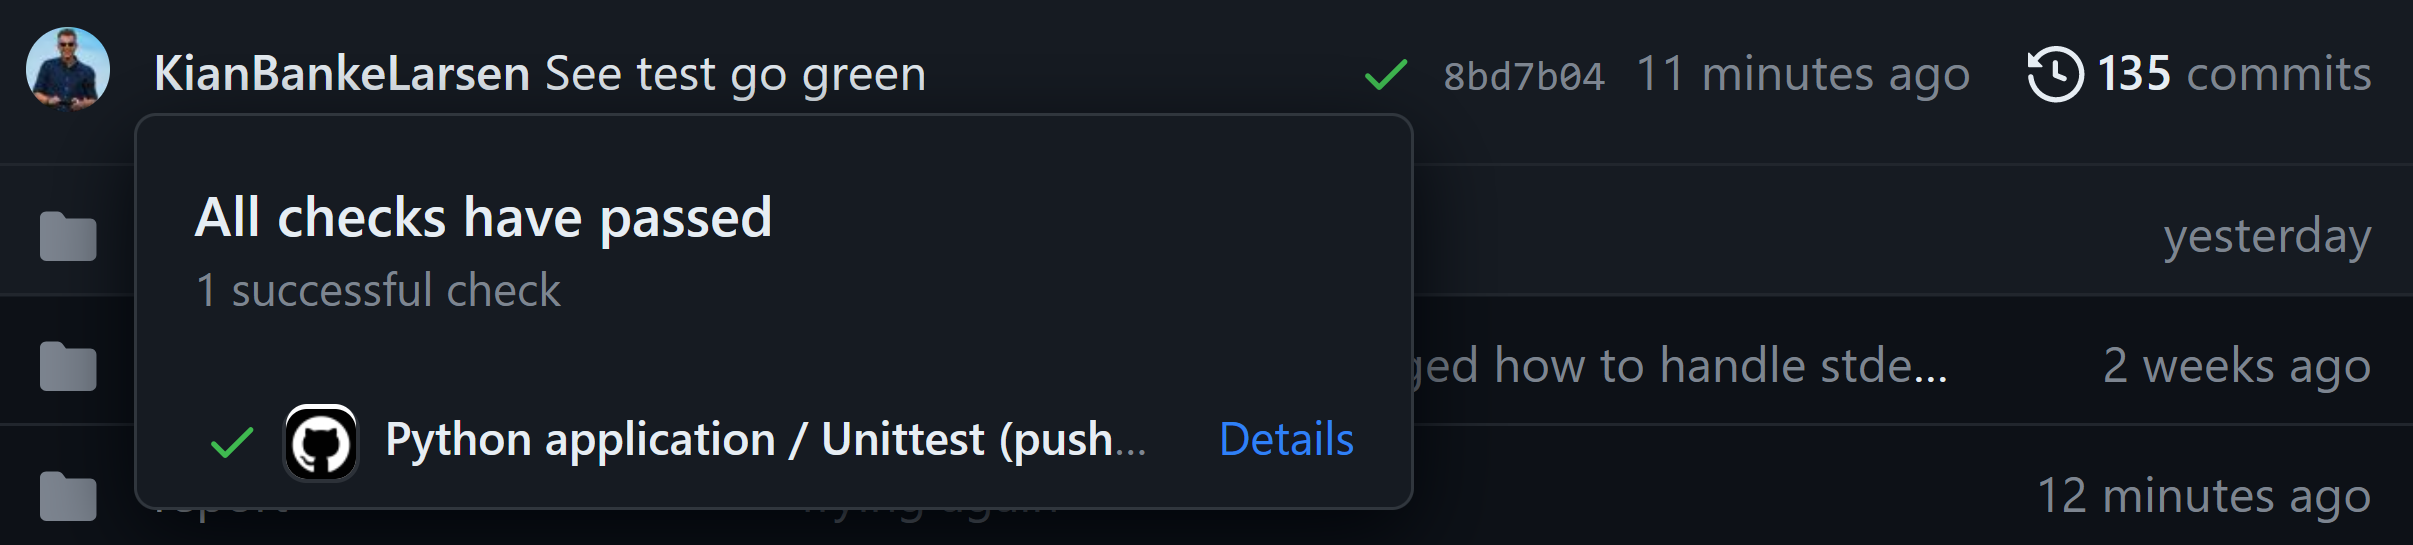
\includegraphics[width=1\textwidth]{misc/images/GitHub_Actions.png}
    \caption{GitHub Actions for system testing.}
\end{figure}

That way, one know exactly which push or pull request caused the tests to fail, and associated code is directly available from the workflow via commit ID. History for workflow is available too.

\begin{figure}[H]
    \centering
    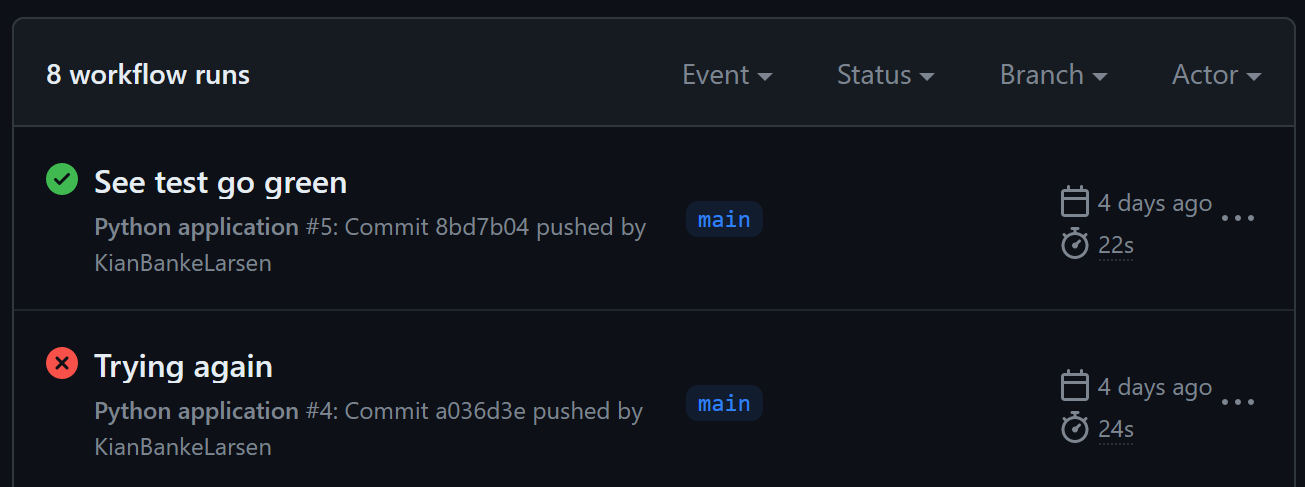
\includegraphics[width=1\textwidth]{misc/images/Workflow.png}
    \caption{Workflow history.}
\end{figure}

A workflow build consists of the stages stated in Figure \ref{fig:workflow_run}.  Note that, in this example, the stack machine test passed, but the register version did not. Upon build failure, an email is sent to whom introduced the issue.

\begin{figure}[H]
    \centering
    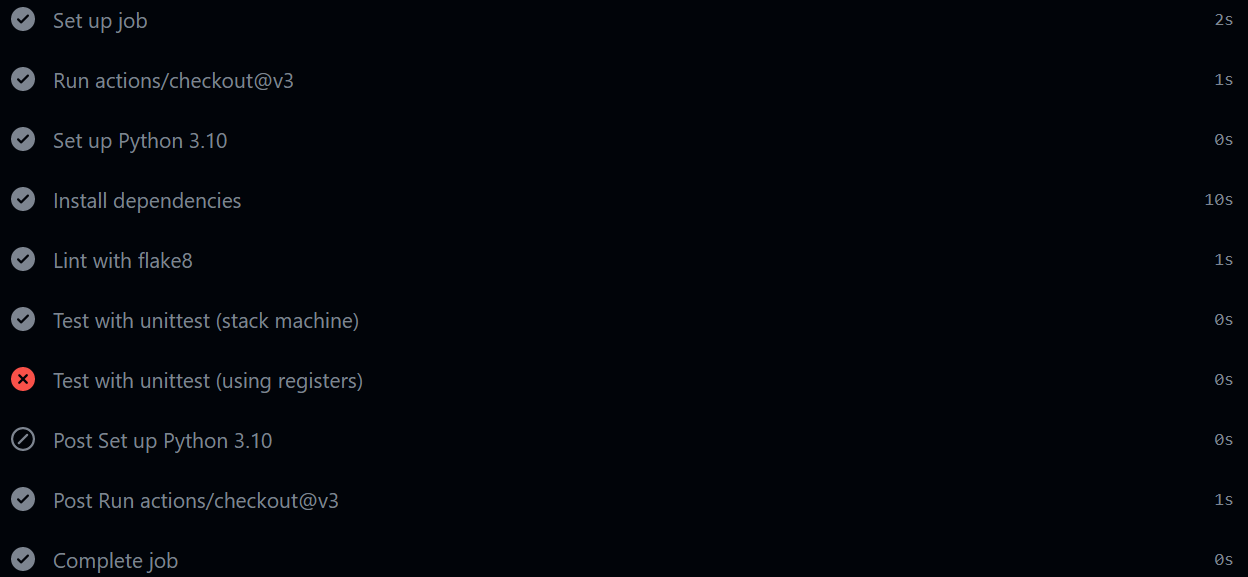
\includegraphics[width=1\textwidth]{misc/images/workflow_run.png}
    \caption{Workflow run. Red indicates failure.}
    \label{fig:workflow_run}
\end{figure}

The list of tests is too long to mention each one, instead three tests that caused particularly many problems have been chosen. The tests are representative because they have a relatively high complexity, as the input programs utilize recursion, loops and nested scopes. For this to work properly, it requires that the constructs and static link pointer works correctly. In addition, it must be possible to tear down several stack frames at once, since every scope introduces a new stack frame. Failing to remove a stack frame properly causes problems in the \texttt{postreturn} and \texttt{epilog} phase, and in worst case segmentation fault. 

The test below is borrowed from SCIL. The test is named summers.panda.

\begin{minted}{c}
int sum_recurse(int n) {
    if(n == 1) {return 1;} else {
        return n + sum_recurse(n - 1);
    }
}
int sum_loop(int n) {
    int sum, i;
    i = 1; sum = 0;
    while(i <= n) {
        sum = sum + i;
        i = i + 1;
    }
    return sum;
}

print(sum_recurse(9)); print(sum_loop(9));
print(sum_recurse(42)); print(sum_loop(42));
\end{minted}

The test below does not calculate anything meaningful or difficult, but it checks that the functionality implemented in Figure \ref{fig:remove_stack_frames} works as expected.

\begin{minted}{c}
int i = 5;
int main(){
    if(1){
        if(1){
            if(1){
                i = i + 1;
                return i;
            }
        }
    }
}
print(main());
\end{minted}

The goal has been to test all legal semantics thoroughly. This includes assignment to variables declared outside the current scope. Assignment to formal parameters, recursion, return from static nested scopes, comments, sugared declaration with assignment, binary operations (comparisons and arithmetic) and constructs like \texttt{while}, \texttt{for}, \texttt{if} and \texttt{print}.

A test that is particularly critical for the register machine is right-unbalanced trees,\footnote{This is tested with the test cases \texttt{/testing/test-cases/unbalanced\_right\_addition.panda} and \texttt{/testing/test-cases/unbalanced\_right\_subtraction.panda}.} or complete trees, because these cause a greater register need. An example of such tree can be found in Figure \ref{fig:unbalanced_tree}. The figure is part of the syntax tree for the input program given below:

\begin{minted}{c}
print(1+(1+(1+(1+(1+(1+(1+(1+(1+(1+(1+(1+(1+(1))))))))))))));
\end{minted}

The reason is, in this case, that the left child is always visited first, after which the expression in the right child must be evaluated. This is clear in Figure \ref{fig:binop}. It is therefore necessary to preserve all left children until there are no more right children. In the case of the stack machine, this is not something one think too much about, as the stack just grows as expected. With register allocation, attention is required, because there must be a place to store values, since these must be in a register, regardless of whether this register is spilled onto the stack, it is still a ``register".

\begin{figure}[H]
    \centering
    \digraph[scale=0.5]{rightTree}{
	3 [label=1]
	4 [label=1]
	5 [label=1]
	6 [label=1]
	7 [label="..."]
	8 [label="+"]
	8 -> 6
	8 -> 7
	9 [label="+"]
	9 -> 5
	9 -> 8
	10 [label="+"]
	10 -> 4
	10 -> 9
	11 [label="+"]
	11 -> 3
	11 -> 10
	12 [label=print]
	12 -> 11
}

    \caption{Unbalanced expression.} 
    \label{fig:unbalanced_tree}
\end{figure}

To be precise, the input program uses 27 temporary registers as a consequence of the code generation, which after preparation of the interference graph and coloring can be stored in 14 physical registers. The Emit phase only provides 9 registers for storage, meaning that 5 registers are located on the stack.


\section{Coverage}
Coverage cannot and should not be a measure of test quality, because the order in which functions and flow are executed has a great influence on the result. However, code coverage gives a direct warning if subsets of the code have not been tested at all. Thus, it is clear that more tests need to be written.

The code coverage measuring tool \texttt{coverage.py} is used to perform code coverage statistics on this project. Code coverage is performed in the following way:

\begin{minted}{text}
Compiler$ python3.10 -m coverage erase
    && python3.10 -m coverage run -a main.py -td
    && python3.10 -m coverage run -a main.py -tsd 
    && python3.10 -m coverage report 

Name                                     Stmts   Miss  Cover
------------------------------------------------------------
main.py                                     24      2    92%
src/compiler.py                             70      3    96%
src/dataclass/AST.py                       125      0   100%
src/dataclass/iloc.py                       22      0   100%
src/dataclass/symbol.py                     36      2    94%
src/enums/code_generation_enum.py           38      0   100%
src/enums/symbols_enum.py                    5      0   100%
src/phase/allocator.py                     213      5    98%
src/phase/code_generation_base.py           58      3    95%
src/phase/code_generation_register.py      262      9    97%
src/phase/code_generation_stack.py         199      5    97%
src/phase/emit.py                          199     17    91%
src/phase/lexer.py                          44      8    82%
src/phase/parser.py                        101      2    98%
src/phase/parsetab.py                       18      0   100%
src/phase/symbol_collection.py             117      2    98%
src/phase/syntactic_desugaring.py           65      0   100%
src/printer/ast_printer.py                 141      3    98%
src/printer/generic_printer.py              17      0   100%
src/printer/symbol_printer.py               40      0   100%
src/utils/error.py                           5      0   100%
src/utils/interfacing_parser.py              1      0   100%
src/utils/label_generator.py                 7      0   100%
src/utils/x86_instruction_enum_dict.py       2      0   100%
testing/test.py                             75      0   100%
------------------------------------------------------------
TOTAL                                     1884     61    97%
Wrote HTML report to htmlcov/index.html
\end{minted}

Based on this output, it can be assessed that the prepared tests in the \texttt{test-cases} folder cover the code well. Note that code coverage is run with the debug flag, \texttt{-d}. This is because code in the printer files are only executed when debug is desired.

It is possible to convert the coverage data to an HTML report with the command \texttt{python3.10 -m coverage html}. The advantage of having the data in report form is that it is possible to see which lines have been executed and which are missing, as shown in the figure below: 

\begin{figure}[H]
    \centering
    \begin{subfigure}{1\textwidth}
        \centering
        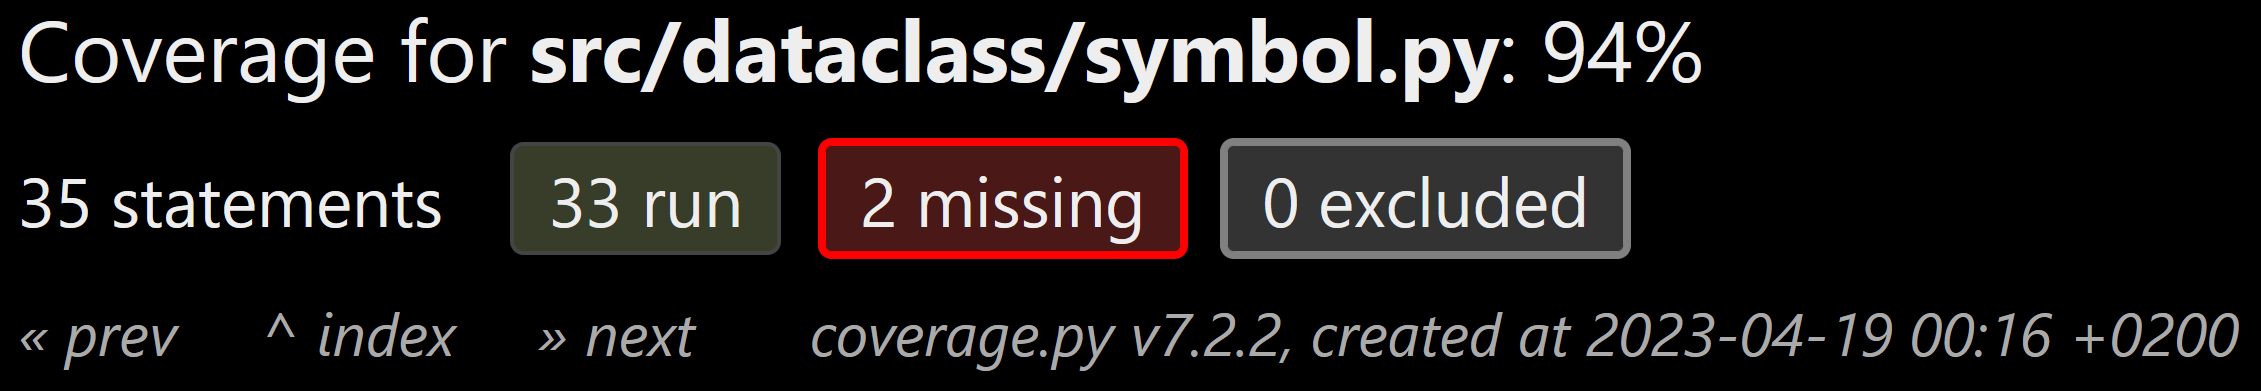
\includegraphics[width=1\textwidth]{misc/images/Coverage_Panel.png}
        \end{subfigure}\\
        \begin{subfigure}{1\textwidth}
        \centering
        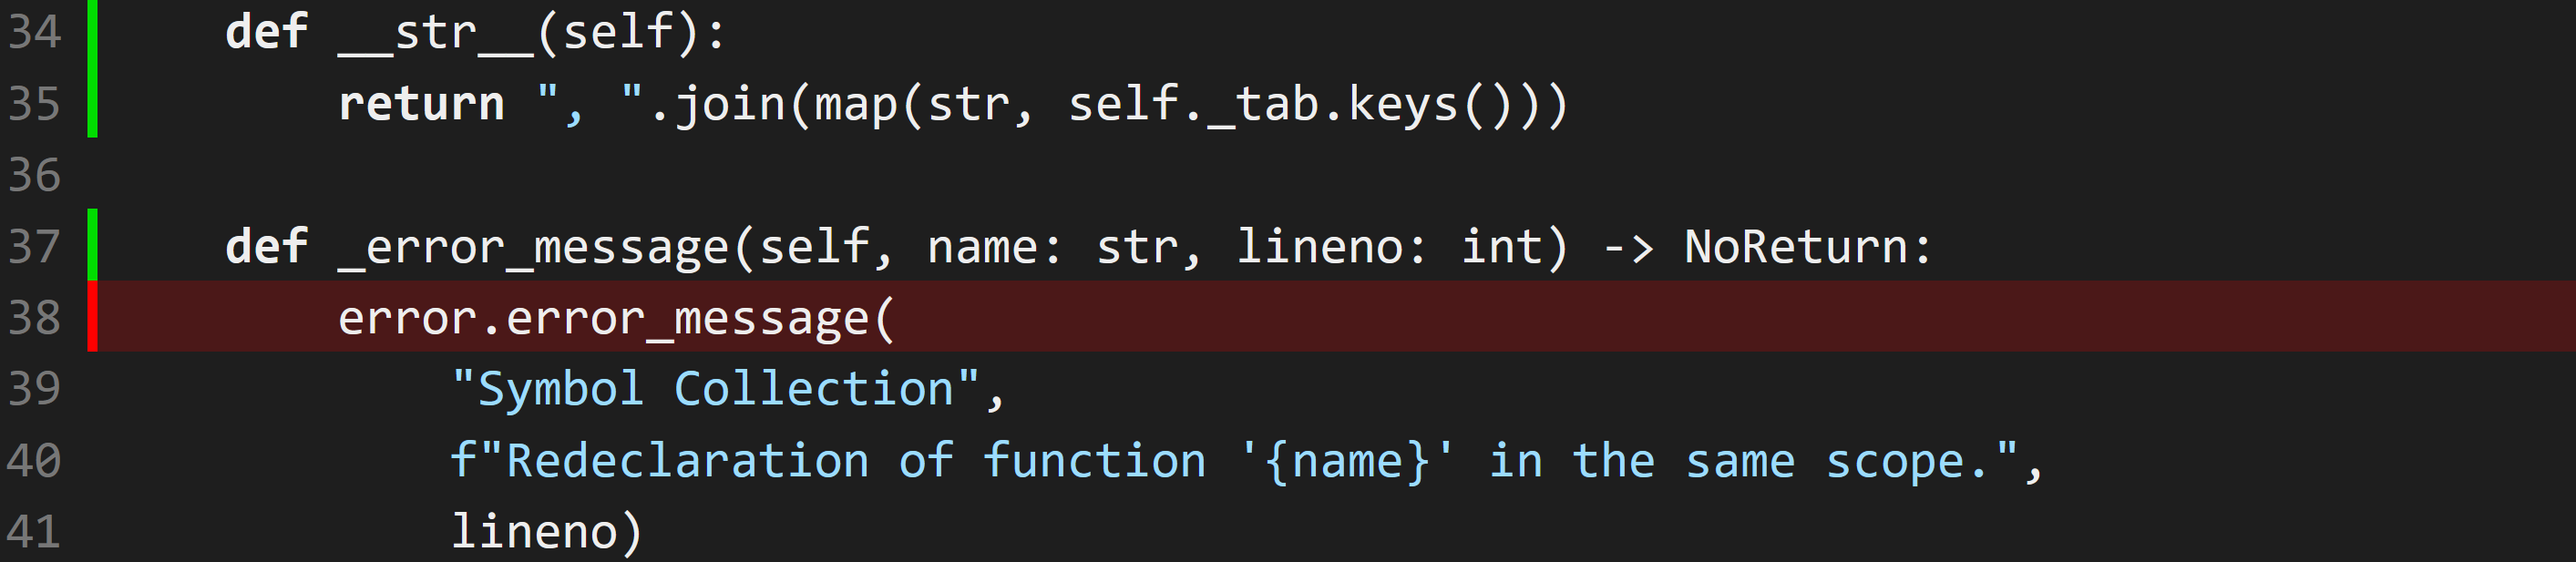
\includegraphics[width=1\textwidth]{misc/images/Coverage_Info.png}
        \end{subfigure}
    \caption{Coverage HTML report.}
\end{figure}

The HTML report also makes it possible to carry out filtering etc. in the file overview table, and thus get a nicer and more user-friendly interface.

\chapter{Performance Comparison}
introduction...

\begin{figure}[H]
    \centering
    \pgfplotstableread[row sep=\\,col sep=&]{
test & stack & register \\                                         
%sum\_recurse(30000) & 21 & 21 \\                                          
sum\_loop(300000000) & 1461 & 858 \\                                         
fibonacci(39) & 2159 & 1648 \\                                                                              
for-loop & 2361 & 852 \\                     
}\mybardata
\begin{tikzpicture}
    \begin{axis}[
        ybar,
        ylabel=Milliseconds,
        ymajorgrids=true,
        xtick pos=lower,
        %xticklabel style={rotate=90},
        %ytick pos=left,
        grid style=dashed,
        width=1\linewidth,
        xlabel=Test,
        title = Milliseconds vs Test,
        bar width=.6cm,
        legend style={at={(0.05,.95)},anchor=north west},
        symbolic x coords={sum\_loop(300000000),fibonacci(39), for-loop},
        xtick=data,
    ]
    \addplot+[color=blueplot] table[x=test,y=register]{\mybardata};
    \addplot+[color=redplot] table[x=test,y=stack]{\mybardata};
    \legend{Register, Stack}
    \end{axis}
\end{tikzpicture}
    \caption{Stack Machine vs Register Machine.}
    \label{fig:performance_comparison}
\end{figure}

\newpage

second page...


\chapter{Evaluation}
This chapter is devoted to reflecting on the learning through the project, as well as describing some issues that could be interesting to work on if the project had had a longer duration.

\section{Retrospect}
There are two fundamental principles that must be observed when building a compiler. The first principle is inviolable:

\begin{displayquote}
    \textit{``The compiler must preserve the meaning of the input program.''}
\end{displayquote}
\hspace*\fill{\small--- \cite[6]{EnginneringACompiler}}

The second principle has a more practical aspect:

\begin{displayquote}
    \textit{``The compiler must discernibly improve the input program.''}
\end{displayquote}
\hspace*\fill{\small--- \cite[7]{EnginneringACompiler}}

It has been a core value throughout the project to make a well-defined compiler implementation that does not do anything inappropriate. Furthermore, the goal has been to create a clear, consistent, easily understandable grammar that a user would be able to pick up with ease. It is assessed that the first principle has been complied with. In this project, no special effort has been made in optimization apart from the preparation of an implementation that uses registers, which is why the second principle must be trivially respected. An example of an optimization that could challenge this would be instruction scheduling, since instructions are literally rescheduled after the invariant based linear IR has been generated.

The approach to the project has been academically based on literature, in order to gain an overview of new as well as old knowledge. Although this has given a confident approach to the project, it must be recognized that it has dulled the process unnecessarily. When coding a project such as a compiler that consists of relatively many lines of code, and many hours of debugging, it is necessary to purposefully choose a theme and then learn as needed, otherwise many hours are lost on something that is not directly applicable. The hours are of course not wasted, but not beneficial for the project either.

It has always been desired that it should be possible to declare new variables in any scope, which is why it was decided to let \texttt{body} (syntactic category from parsing) be what constituted a scope. The choice later made it clear, during code generation phase, that this imposed too many constraints on how the stack should be set up, since a simple generalized procedure linkage was wanted. This resulted in suddenly having to handle all scopes as procedure calls, though it had nothing to with a procedure call. One also encounter problems when doing local register allocation, because flow is only considered locally for a scope (normally local to functions). This consequence limits the analysis to the individual scope, making the content of a \texttt{then} block, of an \texttt{if}-statement, a black box for the surrounding scope. Thus, the analysis of control flow becomes less effective, which contributes to overall poorer performance of the register machine compiler. The easiest solution, and most likely most effective, would be to redo the scope implementation. Global register allocation would be the hard option, though it would not solve the underlying problem besides patching it.

\section{Further Development}

\newpage

\section{Single Point Of Contact}
As a final rounding and summary of the project, GitHub Pages have been used as an addendum to the report, hoping to provide a brief user-friendly introduction to the code and the report. A screenshot of the website can be found in Figure \ref{fig:GitHub_Pages}.

The website has been created with Jekyll, which is a tool that can automatically transform plain text into a static website. The tool only requires a small YAML file (\texttt{/\_config.yml}), listed below, and a markdown file for the page's content.

\begin{minted}{yaml}
theme: jekyll-theme-slate
title: Panda Compiler
description: This is a bachelor project, Southern University of Denmark
show_downloads: true
\end{minted}

The website is simply a nice presentation of the \texttt{README.md} file. In addition, it is possible to download the project directly here, or follow the link to GitHub.

\begin{figure}[H]
    \centering
    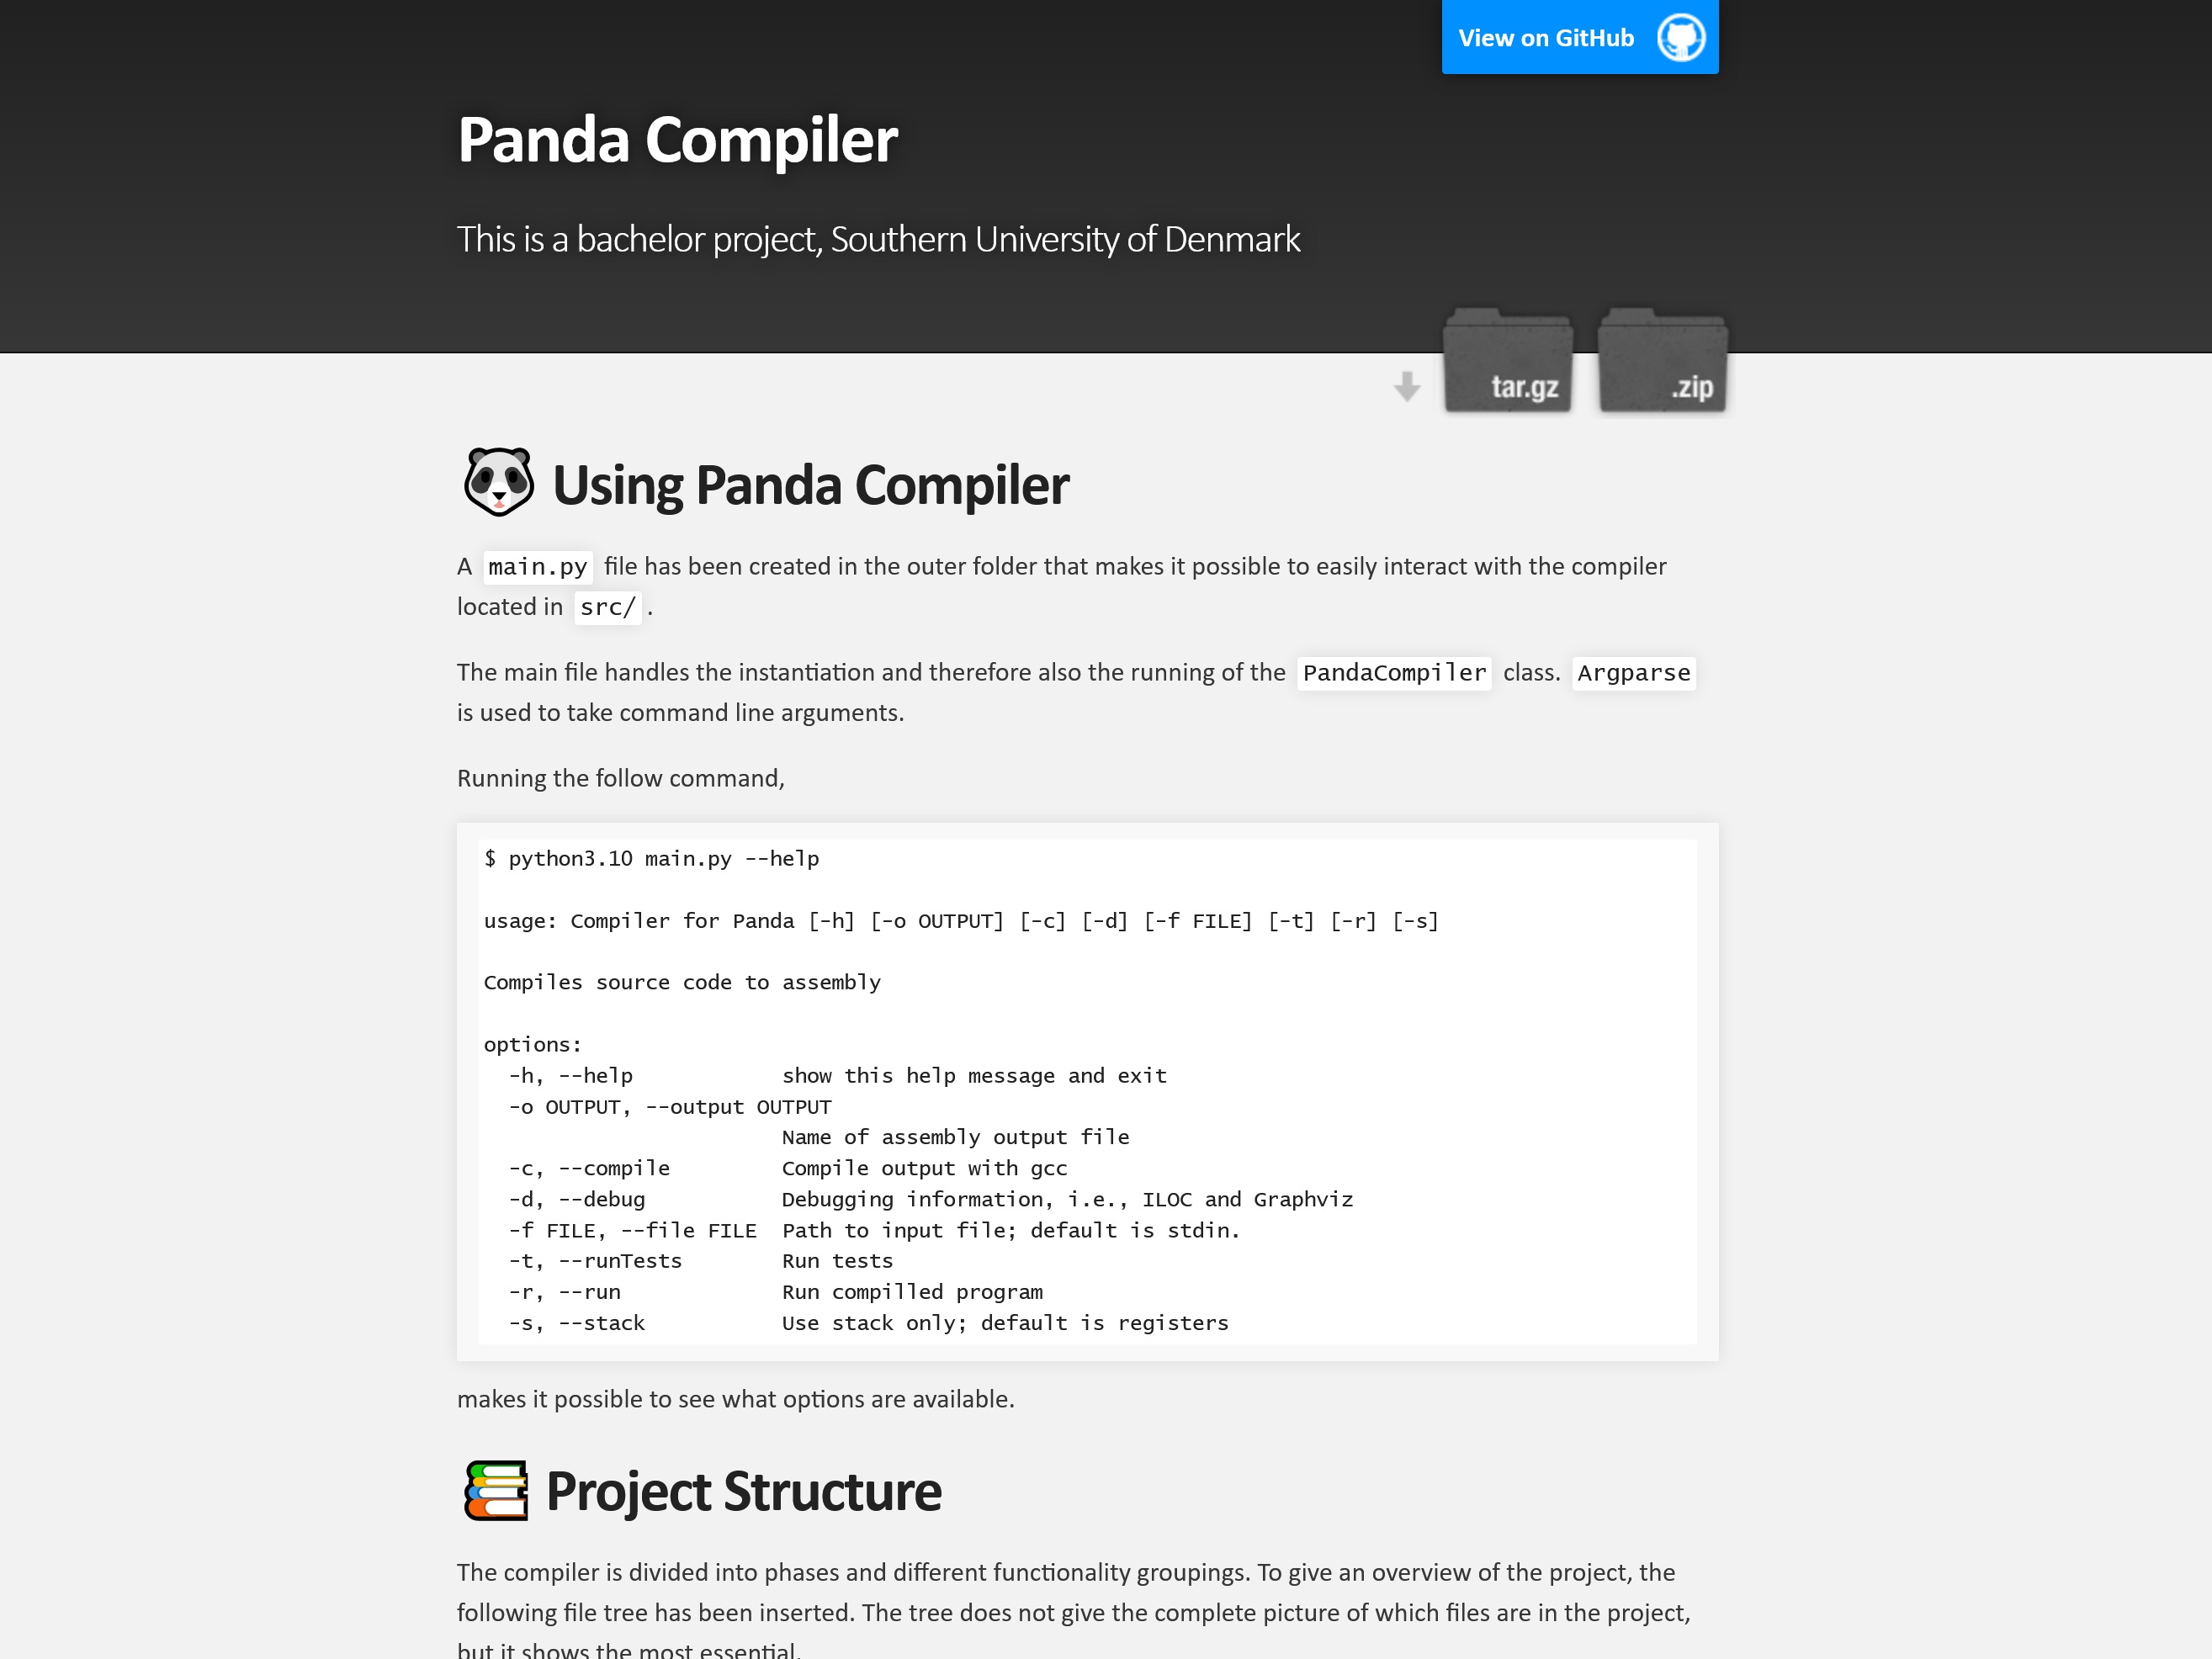
\includegraphics[width=1\textwidth]{misc/images/GitHub_Pages.png}
    \caption{Automatically generated Jekyll Slate website hosted on GitHub Pages: \url{https://kianbankelarsen.github.io/Compiler/}.}
    \label{fig:GitHub_Pages}
\end{figure}

GitHub Pages takes care of deployment when a YAML is specified. Subsequently, the website will be automatically deployed on any push to GitHub -- at the same time as the workflow for testing runs.

\chapter{Conclusion}

\cleardoublepage
\phantomsection
\addcontentsline{toc}{chapter}{References}
\printbibliography
\end{document}